% vim: set textwidth=120:

% Example CV based on the 1.5-column-cv template. Main features:
% * uses the Roboto font family and IcoMoon icon set;
% * doesn't use colours, different font weights are used instead for styling;
% * because the CV fits on one page, header and footer is empty, since there isn't much useful info to put there;
% * includes a photo.
\documentclass[a4paper,10pt]{article}


% package imports
% ---------------

\usepackage[british]{babel} % for correct language and hyphenation and stuff
\usepackage{calc}           % for easier length calculations (infix notation)
\usepackage{enumitem}       % for configuring list environments
\usepackage{fancyhdr}       % for setting header and footer
\usepackage{fontspec}       % for fonts
\usepackage{geometry}       % for setting margins (\newgeometry)
\usepackage{graphicx}       % for pictures
\usepackage{microtype}      % for microtypography stuff
\usepackage{xcolor}         % for colours


% margin and column widths
% ------------------------

% margins
\newgeometry{left=15mm,right=15mm,top=15mm,bottom=15mm}

% width of the gap between left and right column
\newlength{\cvcolumngapwidth}
\setlength{\cvcolumngapwidth}{3.5mm}

% left column width
\newlength{\cvleftcolumnwidth}
\setlength{\cvleftcolumnwidth}{44.5mm}

% right column width
\newlength{\cvrightcolumnwidth}
\setlength{\cvrightcolumnwidth}{\textwidth-\cvleftcolumnwidth-\cvcolumngapwidth}

% set paragraph indentation to 0, because it screws up the whole layout otherwise
\setlength{\parindent}{0mm}


% style definitions
% -----------------
% style categories explanation:
% * \cvnameXXX is used for the name;
% * \cvsectionXXX is used for section names (left column, accompanied by a horizontal rule);
% * \cvtitleXXX is used for job/education titles (right column);
% * \cvdurationXXX is used for job/education durations (left column);
% * \cvheadingXXX is used for headings (left column);
% * \cvmainXXX (and \setmainfont) is used for main text;
% * \cvruleXXX is used for the horizontal rules denoting sections.

% font families
\defaultfontfeatures{Ligatures=TeX} % reportedly a good idea, see https://tex.stackexchange.com/a/37251

\newfontfamily{\cvnamefont}{Roboto Medium}
\newfontfamily{\cvsectionfont}{Roboto Medium}
\newfontfamily{\cvtitlefont}{Roboto}
\newfontfamily{\cvdurationfont}{Roboto Light Italic}
\newfontfamily{\cvheadingfont}{Roboto}
\setmainfont{Roboto Light}

% colours
\definecolor{cvnamecolor}{HTML}{000000}
\definecolor{cvsectioncolor}{HTML}{000000}
\definecolor{cvtitlecolor}{HTML}{000000}
\definecolor{cvdurationcolor}{HTML}{000000}
\definecolor{cvheadingcolor}{HTML}{000000}
\definecolor{cvmaincolor}{HTML}{000000}
\definecolor{cvrulecolor}{HTML}{000000}

\color{cvmaincolor}

% styles
\newcommand{\cvnamestyle}[1]{{\Large\cvnamefont\textcolor{cvnamecolor}{#1}}}
\newcommand{\cvsectionstyle}[1]{{\normalsize\cvsectionfont\textcolor{cvsectioncolor}{#1}}}
\newcommand{\cvtitlestyle}[1]{{\large\cvtitlefont\textcolor{cvtitlecolor}{#1}}}
\newcommand{\cvdurationstyle}[1]{{\small\cvdurationfont\textcolor{cvdurationcolor}{#1}}}
\newcommand{\cvheadingstyle}[1]{{\normalsize\cvheadingfont\textcolor{cvheadingcolor}{#1}}}


% inter-item spacing
% ------------------

% vertical space after personal info and standard CV items
\newlength{\cvafteritemskipamount}
\setlength{\cvafteritemskipamount}{5mm plus 1.25mm minus 1.25mm}

% vertical space after sections
\newlength{\cvaftersectionskipamount}
\setlength{\cvaftersectionskipamount}{2mm plus 0.5mm minus 0.5mm}

% extra vertical space to be used when a section starts with an item with a heading (e.g. in the skills section),
% so that the heading does not follow the section name too closely
\newlength{\cvbetweensectionandheadingextraskipamount}
\setlength{\cvbetweensectionandheadingextraskipamount}{1mm plus 0.25mm minus 0.25mm}


% intra-item spacing
% ------------------

% vertical space after name
\newlength{\cvafternameskipamount}
\setlength{\cvafternameskipamount}{3mm plus 0.75mm minus 0.75mm}

% vertical space after personal info lines
\newlength{\cvafterpersonalinfolineskipamount}
\setlength{\cvafterpersonalinfolineskipamount}{2mm plus 0.5mm minus 0.5mm}

% vertical space after titles
\newlength{\cvaftertitleskipamount}
\setlength{\cvaftertitleskipamount}{1mm plus 0.25mm minus 0.25mm}

% value to be used as parskip in right column of CV items and itemsep in lists (same for both, for consistency)
\newlength{\cvparskip}
\setlength{\cvparskip}{0.5mm plus 0.125mm minus 0.125mm}

% set global list configuration (use parskip as itemsep, and no separation otherwise)
\setlist{parsep=0mm,topsep=0mm,partopsep=0mm,itemsep=\cvparskip}


% CV commands
% -----------

% creates a "personal info" CV item with the given left and right column contents, with appropriate vertical space after
% @param #1 left column content (should be the CV photo)
% @param #2 right column content (should be the name and personal info)
\newcommand{\cvpersonalinfo}[2]{
    % left and right column
    \begin{minipage}[t]{\cvleftcolumnwidth}
        \vspace{0mm} % XXX hack to align to top, see https://tex.stackexchange.com/a/11632
        \raggedleft #1
    \end{minipage}% XXX necessary comment to avoid unwanted space
    \hspace{\cvcolumngapwidth}% XXX necessary comment to avoid unwanted space
    \begin{minipage}[t]{\cvrightcolumnwidth}
        \vspace{0mm} % XXX hack to align to top, see https://tex.stackexchange.com/a/11632
        #2
    \end{minipage}

    % space after
    \vspace{\cvafteritemskipamount}
}

% typesets a name, with appropriate vertical space after
% @param #1 name text
\newcommand{\cvname}[1]{
    % name
    \cvnamestyle{#1}

    % space after
    \vspace{\cvafternameskipamount}
}

% typesets a line of personal info beginning with an icon, with appropriate vertical space after
% @param #1 parameters for the \includegraphics command used to include the icon
% @param #2 icon filename
% @param #3 line text
\newcommand{\cvpersonalinfolinewithicon}[3]{
    % icon, vertically aligned with text (see https://tex.stackexchange.com/a/129463)
    \raisebox{.5\fontcharht\font`E-.5\height}{\includegraphics[#1]{#2}}
    % text
    #3

    % space after
    \vspace{\cvafterpersonalinfolineskipamount}
}

% creates a "section" CV item with the given left column content, a horizontal rule in the right column, and with
% appropriate vertical space after
% @param #1 left column content (should be the section name)
\newcommand{\cvsection}[1]{
    % left and right column
    \begin{minipage}[t]{\cvleftcolumnwidth}
        \raggedleft\cvsectionstyle{#1}
    \end{minipage}% XXX necessary comment to avoid unwanted space
    \hspace{\cvcolumngapwidth}% XXX necessary comment to avoid unwanted space
    \begin{minipage}[t]{\cvrightcolumnwidth}
        \textcolor{cvrulecolor}{\rule{\cvrightcolumnwidth}{0.3mm}}
    \end{minipage}

    % space after
    \vspace{\cvaftersectionskipamount}
}

% creates a standard, multi-purpose CV item with the given left and right column contents, parskip set to cvparskip
% in the right column, and with appropriate vertical space after
% @param #1 left column content
% @param #2 right column content
\newcommand{\cvitem}[2]{
    % left and right column
    \begin{minipage}[t]{\cvleftcolumnwidth}
        \raggedleft #1
    \end{minipage}% XXX necessary comment to avoid unwanted space
    \hspace{\cvcolumngapwidth}% XXX necessary comment to avoid unwanted space
    \begin{minipage}[t]{\cvrightcolumnwidth}
        \setlength{\parskip}{\cvparskip} #2
    \end{minipage}

    % space after
    \vspace{\cvafteritemskipamount}
}

% typesets a title, with appropriate vertical space after
% @param #1 title text
\newcommand{\cvtitle}[1]{
    % title
    \cvtitlestyle{#1}

    % space after
    \vspace{\cvaftertitleskipamount}
    % XXX need to subtract cvparskip here, because it is automatically inserted after the title "paragraph"
    \vspace{-\cvparskip}
}


% header and footer
% -----------------

% set empty header and footer
\pagestyle{empty}



% preamble end/document start
% ===========================

\begin{document}


% personal info
% -------------

\cvpersonalinfo{
    % photo
    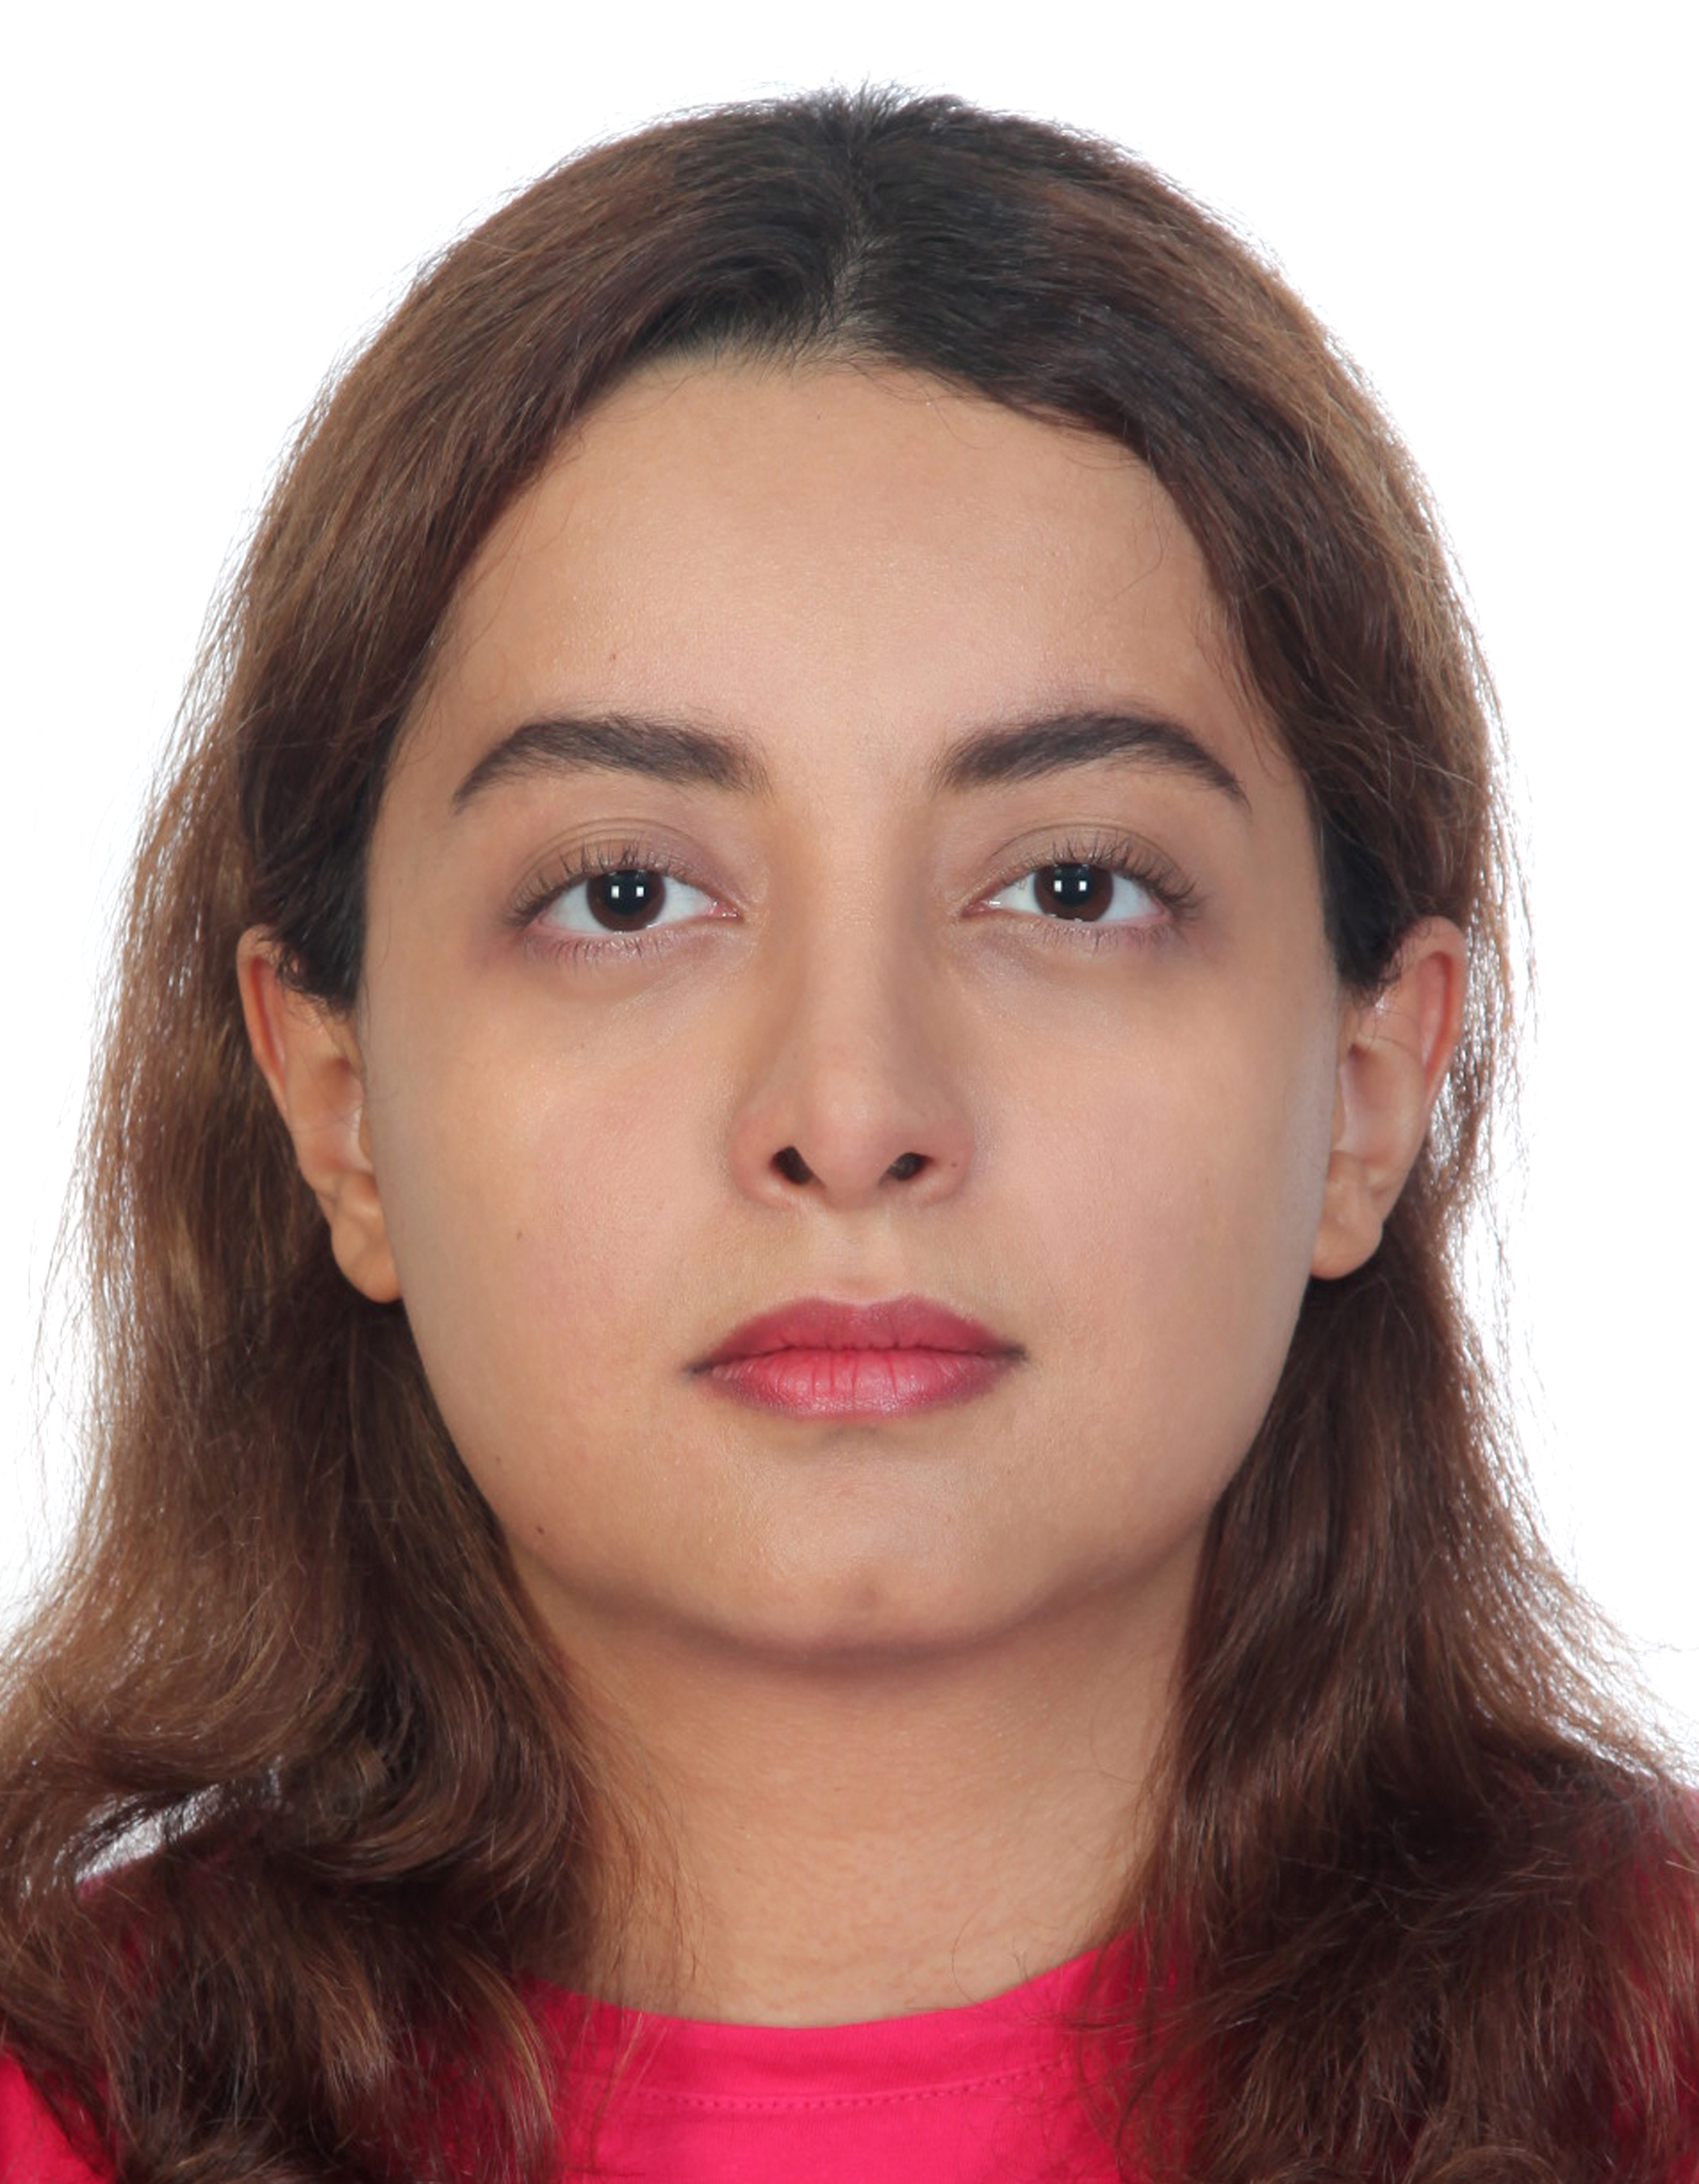
\includegraphics[height=36mm]{PassportPhoto.jpg}
}{
    % name
    \cvname{FATEMEH KARIMI BARIKARASFI}

    % address
    \cvpersonalinfolinewithicon{height=4mm}{072-location.pdf}{
        Tehran, Iran
    }

    % phone number
    \cvpersonalinfolinewithicon{height=4mm}{067-phone.pdf}{
        00989337946278
    }

    % email address
    \cvpersonalinfolinewithicon{height=4mm}{070-envelop.pdf}{
        fatemehkarimi2178@gmail.com
    }

    % LinkedIn account
    \cvpersonalinfolinewithicon{height=4mm}{458-linkedin.pdf}{
        fatemehkarimi2178
    }

    % date of birth
    % Born 14 March 1985
}

% education
% ---------
\cvsection{Education}
\cvitem{
    \cvdurationstyle{ Sept. 2017- Jan. 2022}
}{
    \cvtitle{{Iran University of Science and Technology} \hfill{\textnormal{\textit{Tehran, Iran}}}}
    B.Sc in Electrical Engineering (Telecommunication)
    \begin{itemize}[leftmargin=*]
        \item GPA: 15.92/20
        \item Last two years GPA: 16.53/20
    \end{itemize}
}

\cvitem{
    \cvdurationstyle{June. 2016- Aug. 2016}
}{
    \cvtitle{{Young Scholar Club} \hfill{\textnormal{\textit{Tehran, Iran}}}}
    Physics
    \begin{itemize}[leftmargin=*]
        \item Got Bronze Modal in 29th National Physics Olympiad
    \end{itemize}
}

\cvitem{
    \cvdurationstyle{ Sept. 2013 - June. 2017}
}{
    \cvtitle{{Farzanegan2 High School} \hfill{\textnormal{\textit{Tehran, Iran}}}}
    Diploma in Mathematics and Physics
    \begin{itemize}[leftmargin=*]
        \item Pre-university GPA: 18.86/20
        \item Senior High School GPA: 17.86/20
    \end{itemize}
}

% Research Interest
\cvsection{Research Interest}
\cvitem{\;}{
    \begin{itemize}[leftmargin=*]
        \item Theoretical Physics
        \item Mathematics and Statistics
        \item Computational Neuroscience
        \item Signal Processing
    \end{itemize}
}
% education
% ---------

\cvsection{Research Experience}
\cvitem{
    \cvdurationstyle{Apr. 2021 - Oct. 2021}
}{
    \cvtitle{{Undergraduate Research Assistant} \hfill{\textnormal{\textit{Tehran, Iran}}}}
    {Department of Electrical Engineering, Iran University of Science and Technology}
    \begin{itemize}[leftmargin=*]
        \item Worked on Routing algorithms analysis (Dijkstra, Bellman-Ford, and Q-Routing) on Static and
              Dynamically Changed Networks modeled by Queuing Theory
              \newline
              \textit{\small{Under the supervision of Prof. Shahrokh Farahmand}}
              \newline
              \textit{\small{Grade Point: 20/20}}
    \end{itemize}
}

\cvsection{Achievement}
\cvitem{
    \cvdurationstyle{2016 – Ongoing}
}{
    \begin{itemize}[leftmargin=*]
        \item Member of Iran’s National Elites Foundation
    \end{itemize}
}
\vspace{-4mm}
\cvitem{
    \cvdurationstyle{2016}
}{
    \begin{itemize}[leftmargin=*]
        \item Received Bronze Medal in Iran’s National Physics Olympiad
    \end{itemize}
}
\vspace{-4mm}
\cvitem{
    \cvdurationstyle{2011 – 2017}
}{
    \begin{itemize}[leftmargin=*]
        \item Member of National Organization for Development of Exceptional Talents
    \end{itemize}
}

% skills
% ------

\cvsection{Technical Skill}
\vspace{\cvbetweensectionandheadingextraskipamount}
\cvitem{
    \cvheadingstyle{Programming Language}
}{
    Python, C/C++, MATLAB
}
\vspace{-4mm}
\cvitem{
    \cvheadingstyle{Framework and Library}
}{
    NumPy, Pandas, Matplotlib, TensorFlow, Keras, Scikit-learn, NetworkX
}
\vspace{-4mm}
\cvitem{
    \cvheadingstyle{Professional Software}
}{
    P–Spice, H–Spice, OMNeT++, HFSS
}
\vspace{-4mm}
\cvitem{
    \cvheadingstyle{Technology}
}{
    Git, VSCode
}

% additional info
% ---------------

\cvsection{Course Project}
\vspace{\cvbetweensectionandheadingextraskipamount}
\cvitem{
    \cvheadingstyle{Linear Control Systems}
}{
    \begin{itemize}[leftmargin=*]
        \item DC motor transfer function estimation \small{\textit{by System Identification Toolbox of MATLAB}}
        \item DC motor position and velocity controller design (Phase-Lag, Phase-Lead, and PID) \small{\textit{by MATLAB}}
    \end{itemize}
}
\cvitem{
    \cvheadingstyle{Digital Communication}
}{
    \begin{itemize}[leftmargin=*]
        \item Implementation of QAM, BPSK, FSK, and Ml modulation and detection algorithms in AWGN Channel \small{\textit{by MATLAB}}
        \item Implementation of QPSK and BPSK modulation and detection algorithms in Rayleigh Fading Channel \small{\textit{by MATLAB}}
        \item Implementation of Hamming code and its detection algorithm in AWGN Channel \small{\textit{by MATLAB}}

    \end{itemize}
}
\cvitem{
    \cvheadingstyle{Digital Signal Processing}
}{
    \begin{itemize}[leftmargin=*]
        \item Implementation of OFDM sender and receiver \small{\textit{by MATLAB}}
        \item Speech signal denoising using implemented FIR and IIR filters  \small{\textit{by MATLAB}}
    \end{itemize}
}
\cvitem{
    \cvheadingstyle{Electronic Circuit}
}{
    \begin{itemize}[leftmargin=*]
        \item Circuit design and simulation of following Electrical Circuits: Voltage Regulator, Electrical Thermometer,
              and several Voltage and Current Amplifiers \small{\textit{by P–Spice}}
        \item Design and simulation of following Integrated Circuits: an Operational Amplifiers, a Current Source,
              and a Folded Cascode Amplifier \small{\textit{by H–Spice}}
    \end{itemize}
}
\cvitem{
    \cvheadingstyle{Economic Engineering}
}{
    \begin{itemize}[leftmargin=*]
        \item Economic evaluation of a homemade solar power plant \small{\textit{by EXCEL}}
    \end{itemize}
}
\cvitem{
    \cvheadingstyle{Antenna}
}{
    \begin{itemize}[leftmargin=*]
        \item Cross Dipole Antenna design, simulation, and analysis \small{\textit{by HFSS}}
    \end{itemize}
}

\cvsection{Online Course}
\cvitem{
    \cvdurationstyle{Dec. 2023 - Apr. 2024}
}{
    \cvtitle{{Machine Learning Specialization} \textit{\small{by Stanford University}}}
    % \textit{by Stanford University}
    % \begin{itemize}[leftmargin=*]
    %     \item {\textbf{Covered Topics}: Supervised Machine Learning, Advanced Learning Algorithms, Unsupervised Learning, Recommenders, Reinforcement Learning}
    % \end{itemize}
}
\vspace{-4mm}
\cvitem{
    \cvdurationstyle{Apr. 2023}
}{
    \cvtitle{{Brain Mapping Spring School} \textit{\small {by National Brain Mapping Laboratory}}}
    % \textit{by National Brain Mapping Laboratory}
    % \begin{itemize}[leftmargin=*]
    %     \item {\textbf{Covered Topics}: Introduction and General Concepts, Introduction to Programming with Python 3, Dynamic Systems and Numerical Integration, Cellular Automata,Lattice Boltzman Modeling of Fluid Flow, Introduction to Discrete Events Simulation, Agent-based Models}
    % \end{itemize}
}

\vspace{-4mm}
\cvitem{
    \cvdurationstyle{Sept. 2022 - Mar. 2023}
}{
    \cvtitle{{Python Programming} \textit{\small{by PYTOPIA}}}
    % \textit{by PYTOPIA}
    % \begin{itemize}[leftmargin=*]
    %     \item {\textbf{Covered Topics}: Object Oriented Programming and Modularization, Advanced Topics including
    %           Decorators, Exceptions, Iterators and Generators, Descriptors, Serialization (JSON, YAML, Pickle), itertools, pytest, concurrency (Thread, Process)}
    % \end{itemize}
}
\vspace{-4mm}
\cvitem{
    \cvdurationstyle{Sept. 2019}
}{
    \cvtitle{{FPGA Course} \textit{\small{by IEEE Student Branch of Iran University of Science and Technology}}}
    % \textit{by IEEE Student Branch of Iran University of Science and Technology}
    % \begin{itemize}[leftmargin=*]
    %     \item {\textbf{Covered Topics}:  Introduction to Verilog and VHDL}
    % \end{itemize}
}

\cvsection{Volunteer Experience}
\cvitem{
    \cvdurationstyle{2019 - Ongoing}
}{
    \cvtitle{{Mathematics and Physics Teacher} \hfill{\textnormal{\textit{Tehran, Iran}}}}
    {}
    \begin{itemize}[leftmargin=*]
        \item Teaching geometry, discrete mathematics, calculus, and physics
    \end{itemize}
}

\cvsection{Reference}
\vspace{\cvbetweensectionandheadingextraskipamount}
\cvitem{
    \cvheadingstyle{Prof. Shahrokh Farahmand}
}{
    {Assistant Professor at Iran University of Science and Technology}
    \begin{itemize}[leftmargin=*]
        \item sha.farahmand@gmail.com
    \end{itemize}
}
\vspace{-4mm}
\cvitem{
    \cvheadingstyle{Prof. Farzan Haddadi}
}{
    {Associate Professor at Iran University of Science and Technology}
    \begin{itemize}[leftmargin=*]
        \item farzanhaddadi@iust.ac.ir
    \end{itemize}
}

\cvsection{Language}
\vspace{\cvbetweensectionandheadingextraskipamount}
\cvitem{
    \cvheadingstyle{English}
}{
    {TOEFL iBT: 93/100 (Reading: 27 | Listening: 28, | Speaking: 19 | Writing: 19)}
}
\vspace{-4mm}
\cvitem{
    \cvheadingstyle{Persian}
}{
    Native
}

\end{document}
